\documentclass[sigconf]{acmart}
\makeatletter
\renewcommand\@formatdoi[1]{\ignorespaces}
\makeatother


\usepackage{booktabs} % For formal tables


% Copyright
%\setcopyright{none}
%\setcopyright{acmcopyright}
%\setcopyright{acmlicensed}
\setcopyright{rightsretained}
%\setcopyright{usgov}
%\setcopyright{usgovmixed}
%\setcopyright{cagov}
%\setcopyright{cagovmixed}

%Conference
\acmConference[H4CK3RS '17]{Proseminar H4ck3r's D3l1ght}{July 2017}{Garching, Bayern}
\acmYear{2017}
\copyrightyear{2017}

%\acmPrice{15.00}


\begin{document}
\title{Designing a modular and expandable compiler}

\author{Jan van Br\"ugge}
\email{jan@vanbruegge.de}

\begin{abstract}
Today's tooling around web technologies has become extremely complex and there are a number of options available. The need for those tools arise out of the move to increasingly client sided web applications. To manage the complexity of those applications, developers use a set of higher level lanugages, that compile down to the native languages of the web: HTML, CSS and Javascript.

    As tooling to combine compilation results is complicated to set up and have a negative impact on end performance caused by adding a runtime, this paper describes a modular compiler with an unified abstract syntax tree (AST). The goal is to plugins to extend the AST definition to allow new syntaxes in existing lanugages with minimal efford. Some lanuages fall in this category, for example is Typescript a superset of ECMAScript2015 (ES6), which is a superset over the old ES5 Javascript standard that is implemented in most browsers.
\end{abstract}

%
% The code below should be generated by the tool at
% http://dl.acm.org/ccs.cfm
% Please copy and paste the code instead of the example below. 
%
\begin{CCSXML}
<ccs2012>
<concept>
<concept_id>10011007.10011006.10011041</concept_id>
<concept_desc>Software and its engineering~Compilers</concept_desc>
<concept_significance>500</concept_significance>
</concept>
<concept>
<concept_id>10011007.10011006.10011041.10011688</concept_id>
<concept_desc>Software and its engineering~Parsers</concept_desc>
<concept_significance>500</concept_significance>
</concept>
</ccs2012>
\end{CCSXML}

\ccsdesc[500]{Software and its engineering~Compilers}
\ccsdesc[500]{Software and its engineering~Parsers}


\keywords{Compilers, Typescript, Javascript}


\maketitle

\section{Introduction}

In modern web development environments, you need to have at least two types of tools:

\begin{itemize}

\item{\textbf{Compilers:} As most browser vendors have not yet implemented the new ES6 standard natively and many developers want to use one of the numerous compile-to-javascript languages that are rising in popularity, you need a compiler to transform the source code into the ES5 Javascript standard, which most browser are able to execute. The most popular compilers are \textit{Babel} for ES6, \textit{TSC} for Typescript and \textit{purs} for Purescript.}

\item{\textbf{Bundlers:} Because until ES6 Javascript did not have a syntax to import modules for other source files and browser vendors have not yet implemented this syntax, you need bundlers that link your code together, provide dependencies and bootstrap your application. Some also generate the \textit{index.html} file with all assets linked or included. The most popular bundler is \textit{webpack}. Other solutions are \textit{rollup} and \textit{browserify}}

\end{itemize}

The seperation between those two creates a few problems:

\begin{itemize}
\item{It is not possible to optimize across modules, because the compiler is not aware of the other modules' AST}

\item{The bundler has to introduce a runtime to wrap the compiled output, because it is not aware of the AST of the code}

\item{It is not easy to use multiple lanugages, especially running tests written in multiple languages is hard as testing tools expect Javacript input}

\item{New syntaxes have to be added to all languages individually, for example JSX which was introduced by Facebook and not usable in Typescript for a long time, because Facebook only implemented support in Babel}

\end{itemize}

The fact that most tools are written in Javascript also leads to problems, because Javascript only has limited concurrency and is slow to execute even with modern virtual machines (VM).

To fix those problems, the goal of this paper is to develop a new compiler whose design allows being extended by modules to add new syntaxes to existing languages with minmal efford. To make implementation easier and performance better, the compiler called \textit{pack.hs} will be written in Haskell.

\section{Design of the compiler}

\subsection{Dynamic AST definition}

The compiler should allow plugins to add syntax to the definitions of other plugins. This means that every plugin, be it a core plugin implementing a certain language like Typescript or an extention plugin that augments existing core plugins, is allowed to add grammar to the AST definition.

One example here would be a JSX plugin on top of a Javascript plugin. JSX is syntax made pobular by Facebook with its React framework. It allows for a HTML-like syntax as a normal Javascript expression, which is used by the framework to describe components to be rendered (see listing~\ref{lst:jsx} as example).

\begin{lstlisting}[caption={Simple JSX view function}, captionpos=b, label=lst:jsx]
function view(state) {
    return (
        <div>
            <span>{ state.myValue }</span>
        </div>
    );
}
\end{lstlisting}

The same syntax is also useful in Typescript, as Typescript is a typed superset of Javascript. So in an ideal case the JSX plugin should work without modifications with both source languages.

As the used plugins are configured at runtime, the final AST definition is not known at runtime. A core plugin should be able to be used together with a extention plugin that was written after the core plugin without having to modify or recompile the core plugin.

To allow this, the compiler only has one abstract data type (ADT) representing a grammar in  augmented Backus--Naur form (ABNF, see listing~\ref{lst:ABNF} as example). The plugins provide grammar files that are then parsed by the compiler to construct the final AST (see section~\ref{sec:pipeline}).

\begin{lstlisting}[linewidth=\columnwidth, caption={Simple example of ABNF grammar}, captionpos=b, label=lst:ABNF]
S ::= function;
function ::= 'function' IDENTIFIER '(' [arguments] ')' block;
arguments ::= argument [additionalArguments];
additionalArguments ::= ',' argument [additionalArguments];
argument ::= IDENTIFIER typeDeclaration | IDENTIFIER;
block ::= '{' statement* '}';
typeDeclaration ::= ':' type;
type ::= 'boolean' | 'string' | 'number';
statement ::= 'return' expression [';'];
literal ::= '"' LITERAL '"' | LITERAL | 'true' | 'false';
expression ::= literal | expression operator expression;
operator ::= '+' | '-' | '===';
\end{lstlisting}

This grammar represents a small subset of Typescript. A similar grammar is used in the current implementation.

\subsection{Compiler pipeline}
\label{sec:pipeline}

A classic compiler is implemented as a pipeline of three to five distinct parts (see figure~\ref{fig:compiler_pipeline}).

\begin{figure}[H]
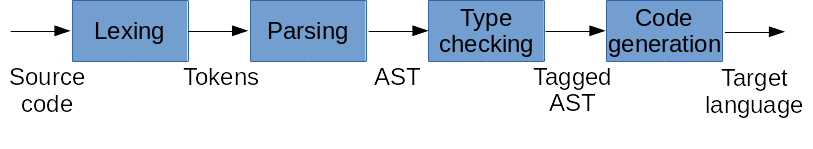
\includegraphics[width=\columnwidth]{./compiler_pipeline.png}
\caption{A classic compiler pipeline}%
\label{fig:compiler_pipeline}
\end{figure}

The lexing step takes the source code to be parsed, together with a Chomsky type 3 grammar that is used to split the raw input string into a ordered set of tokens. This step can be left out, if the characters in the input string are seen as tokens individually.

A Parser then takes those tokens and a Chomsky type 2 grammar to parse an AST\@. This AST can optionally be type checked before it is transformed into the target language. In the context of the web, this most likely Javascript.

In the code generation step, the AST is written into a target file, for Javascript this is another text file. Most of the time this also includes a minification step, where the compiler replaces names with short, obfuscated versions and omits as much whitespace as possible.

The compiler described in this paper also uses a pipeline approach, but with different steps (see figure~\ref{fig:pack.hs_pipeline}).

\begin{figure}[H]
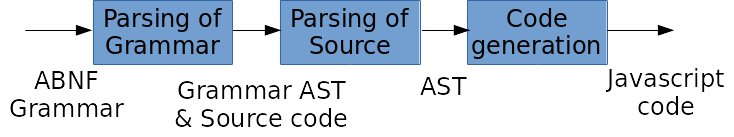
\includegraphics[width=\columnwidth]{./pack_hs_pipeline.png}
\caption{Compiler pipeline in pack.hs}%
\label{fig:pack.hs_pipeline}
\end{figure}

Here the compiler first collects the grammar files from the plugins. In the current proof of concept implementation, this is just one typescript syntax file. Those grammars are then parsed into a special ABNF grammar AST\@.

This AST is then used to generate a source code parser at runtime, which takes the source code and parses it into an AST\@. To simplify the implementation, there is no type checking done yet. This AST is piped through a bunch of transforming functions which come from the plugins. Those transforms are what compiles the code.

The last step again is code generation, which transforms the AST into obfuscated and minified Javascript code.

\section{Implementation}

\subsection{Host language}

The compiler is written in Haskell, because of several advantages:

\begin{itemize}

\item{The lazy nature of Haskell allows for easy parsing of self-recursive grammars}
\item{Later in the project, the compiler can make use of the parallelism built into the Haskell runtime to compile multiple files at the same time.}
\item{Haskell is a compiled language, so the final execution does not suffer performance hits introduced by parsing and interpreting}
\item{Haskell's strong type system makes debugging code a lot easier, because most of the errors are already caught by the compiler}
\item{GHCI, Haskell's interactive interpreting compiler allows to test functions in isolation before inserting them into the program}
\item{The monadic approach and the accompanying \textit{do} notation make composing complex parsers out of simple ones easy}
\item{Parsing libraries for Haskell are feature-rich and very mature, this compiler uses \textit{Megaparsec}}

\end{itemize}

\subsection{Grammar parsing}

To parse the grammar files, the compiler has an ADT representing the AST of a grammar (see listing~\ref{lst:adt_abnf}). The program then uses the \textit{Parser} Monad to pupulate an instance of the ADT.

\begin{lstlisting}[linewidth=\columnwidth, caption={ADT of ABNF grammar}, captionpos=b, label=lst:adt_abnf, language=Haskell]
newtype Grammar = Grammar [Rule]
data Rule = Rule String Production
newtype Production = Production [AlternativeTerm]
newtype AlternativeTerm = AlternativeTerm [Term]
data Term = Many PrimitiveTerm
          | Many1 PrimitiveTerm
          | Primitive PrimitiveTerm
data PrimitiveTerm = Terminal String
                   | NonTerminal String
                   | Optional Production
                   | Group Production
                   | Repetition Int PrimitiveTerm
                   | Identifier
                   | Literal
\end{lstlisting}

As it can be seen above, the \textit{NonTerminal} constructor takes a String instead of a \textit{Rule}, because at rules may reference other rules that are not yet parsed. Initially, there was a matching step after the intial parse, which matched the strings with their respective rules, but the AST would then be a graph, which caused endless loops when trying to postprocess it. Because of this, the rules are matched on the fly by the parser of the source code (see listing~\ref{lst:grammar_match}).

\begin{lstlisting}[linewidth=\columnwidth, caption={Rule matching while parsing}, captionpos=b, label=lst:grammar_match, language=Haskell, breaklines=true]
getRule :: Grammar -> String -> Rule
getRule (Grammar rules) name = head $
    filter (\(Rule n _) -> n == name) rules

parseRule :: Rule -> Grammar -> Parser AST
parseRule (Rule s (Production terms)) g = generateAlternatives terms s g

generatePrimitive :: PrimitiveTerm -> Grammar -> Parser AST
generatePrimitive (NonTerminal name) grammar =
    parseRule (getRule grammar name) grammar
\end{lstlisting}

\subsection{Code generation}

The code generator features a minification step. In this step, all variable and function names are renamed to names that are as short as possible and only necessary whitespace is printed to the target file. The names for the minifier are generated by creating a cartesian product with increasing exponent over the alphaneric characters (see listing~\ref{lst:names}). The first character is choosen only from alphabetic character, because the syntax of Javascript requires this to distinquisch between number literals and indentifiers.

\begin{lstlisting}[linewidth=\columnwidth, caption={Endless list of possible variable names}, captionpos=b, label=lst:names, language=Haskell, breaklines=true]
letters :: [Char]
letters = ['a'..'z'] `mappend` ['A'..'Z'] `mappend` ['$']

alphaNum :: [Char]
alphaNum =  letters `mappend` ['0'..'9']

names :: [String]
names = [ x:xs | i <- [0..],
                 x <- letters,
                 xs <- replicateM i alphaNum
        ]
\end{lstlisting}

\section{Lessons learned}

While building the compiler a few issues surfaced, that are best handled in a rewrite of the current proof of concept. For solutions and ideas about those issues, see section~\ref{sec:future_work}.

\begin{itemize}

\item{The current AST definition is based around strings for everything, which does not allow to use the strong type system of Haskell.}

\item{A unified AST for every language will not work, because to find a common denominator, you loose a lot of the language specific semantics.}

\item{A unified AST is not needed, because per language, there is always a base AST definition that can be extended. For some languages like Javascript and Typescript this is the same base definiton, others like Purescript, that have different language constructs, have their own base AST defintion.}

\end{itemize}

There also where a few positive points about the choosen solutions.

\begin{itemize}

\item{Haskell is an excellent choice as host language for a compiler. The lazyness, especially around infinite lists, makes it a lot easier to parse and transform the AST}

\item{Monadic parsers help a lot with reducing complexity. The parsing libraries for Haskell are powerful, easy to use and very mature. The next iteration of the compiler will use \textit{Megaparsec} again.}

\item{The plugin driven approach can work, if executed correctly. Ideally every plugin would import the compiler for a certain language as library, that other project can also benefit from a Haskell implementation of the compiler.}

\end{itemize}

\section{Future work}
\label{sec:future_work}

A future implementation will not use the double parsing approach. Instead of the current AST defintion (see listing~\ref{lst:ast}) the polymorphic parameter will be used to encode different lanugages. Every node then has an ADT as payload that can be used to encode different types of nodes (see listing~\ref{lst:js_ast}).

\begin{lstlisting}[linewidth=\columnwidth, caption={Current AST defintion}, captionpos=b, label=lst:ast, language=Haskell, breaklines=true]
data GeneralAST a = Node a [GeneralAST a]
         | Leaf a
         | Empty
        deriving (Show)

type AST = GeneralAST String
\end{lstlisting}

\begin{lstlisting}[linewidth=\columnwidth, caption={Example Javascript AST defintion}, captionpos=b, label=lst:js_ast, language=Haskell, breaklines=true]
data GeneralAST a = Node a [GeneralAST a]
         | Empty
        deriving (Show)

data Nodes = Function String [String]
            | Block
            | Statement
            | Expression
            | VarDeclaration String
            | NumLiteral Double
            | BoolLiteral Bool
            | Identifier String
            deriving (Show)

type JavascriptAST = GeneralAST Nodes
\end{lstlisting}

While this is a lot more typesafe than before, the issue now is how to add to the existing defintion of the AST?

For this we can use the technique from \textit{Data types \`a la carte} to allow plugins to add new data types to the original defintion without modifying its source code (see listing~\ref{lst:a_la_carte}).

\begin{lstlisting}[linewidth=\columnwidth, caption={Addition to sum type using type operators}, captionpos=b, label=lst:a_la_carte, language=Haskell, breaklines=true]
{-# LANGUAGE TypeOperators #-}
module AstNew where

-- JsCore.hs
data Tree f = In (f (Tree f))
data (f :+: g) e = Inl (f e) | Inr (g e)

data BoolLiteral e = BoolLiteral Bool

data Block e = Block [e] | SingleStatement e

data VarDeclaration e = VarDeclaration String e

type JavascriptNodes = Block :+: VarDeclaration :+: BoolLiteral

-- JsxExtention.hs
data JsxExpression e = JsxExpression String e

type JsxNodes = JavascriptNodes :+: JsxExpression
\end{lstlisting}

Another, simpler solution could be the use of existential types (see listing~\ref{lst:existential}). With those types, the core plugin only knows that the tree is composed out of types that can be transformed to one of the base Javascript nodes (see listing~\ref{lst:transformable}). This also allows nodes to keep their logical hierachy, for example that a block is composed out of multiple statements (see listing~\ref{lst:is_statement}).

\begin{lstlisting}[linewidth=\columnwidth, caption={Example of an existential type}, captionpos=b, label=lst:existential, language=Haskell, breaklines=true]
{-# LANGUAGE ExistentialQuantification #-}

data AnyShowable = forall a. (Show a) => AnyShowable a

list :: [AnyShowable]
list = [AnyShowable 1, AnyShowable "foo", AnyShowable "bar"]

doShow :: [AnyShowable] -> String
doShow [] = ""
doShow ((AnyShowable x):xs) = show x ++ doShow xs

\end{lstlisting}

\begin{lstlisting}[linewidth=\columnwidth, caption={Existential type for Javascript AST}, captionpos=b, label=lst:transformable, language=Haskell, breaklines=true]
{-# LANGUAGE ExistentialQuantification #-}

data JavascriptNode = Block [ASTNode] | BoolLiteral Bool
data ASTNode = forall a. (TransformableJS a) => ASTNode a

class TransformableJS a where
    transformJS :: a -> JavascriptNode

instance TransformableJS JavascriptNode where
    transformJS = id

instance TransformableJS ASTNode where
    transformJS (ASTNode a) = transformJS a

--JSX.hs
data JSXNodes = --...

instance TransformableJS JSXNodes where
    --Compile JSXNodes here to normal JSNodes

\end{lstlisting}

\begin{lstlisting}[linewidth=\columnwidth, caption={Existential types preserving hierarchy}, captionpos=b, label=lst:is_statement, language=Haskell, breaklines=true]
{-# LANGUAGE ExistentialQuantification #-}

data JavascriptNode = Block [JSStatement]
                    | Statement [ASTNode]
                    | BoolLiteral Bool

data ASTNode = forall a. (TransformableJS a) => ASTNode a
data JSStatement = forall a. (TransformableJS a, IsStatement a) => JSStatement a

class TransformableJS a where
    transformJS :: a -> JavascriptNode

instance TransformableJS JavascriptNode where
    transformJS = id

instance TransformableJS ASTNode where
    transformJS (ASTNode a) = transformJS a

class IsStatement a where
    isStatement :: a -> Bool

instance IsStatement JavascriptNode where
    isStatement (Statement _) = True
    isStatement _ = False

--JSX.hs
data JSXNodes = --...

instance TransformableJS JSXNodes where
    --Compile JSXNodes here to normal JSNodes

\end{lstlisting}

This behavior is very hard to emulate with \textit{Types \`a la carte}, so even if they are more flexible, a future iteration will use existential types to handle all plugins.


\bibliographystyle{ACM-Reference-Format}
\bibliography{sample-bibliography}

\end{document}
